\documentclass{standalone}

\usepackage{graphicx}
\usepackage{tikz}
\usepackage{color}

\newcommand{\hfr}{\ensuremath{h_{23}}}
\newcommand{\rf}{\ensuremath{\mathrm{rf}}}

\begin{document}
\begin{tikzpicture}
    \draw (0, 0) node[inner sep=0] {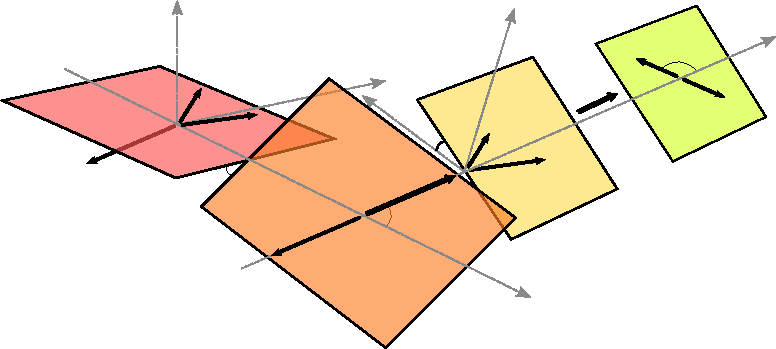
\includegraphics{angles_3b_frames.pdf}};
    \draw (-1.2, -1.5) node {$\vec p_1$};
    \draw (1.8, 1) node {$\vec p_2$};
    \draw (2.9, -0.0) node {$\vec p_3$};
    \draw (0.1, 0.) node {$\vec p_2+\vec p_3$};
    \draw (-2.5, 0.7) node {$\vec p_3$};
    \draw (-2.8, 1.7) node {$\vec p_2$};
    \draw (-5.2, -0.1) node {$\vec p_1$};
    \draw (4.5, 2.2) node {$\vec p_2^{\,*}$};
    \draw (5.7, 0.9) node {$\vec p_3^{\,*}$};
    \draw (5.3, 2.0) node {$\theta_{23}$};
    \draw (0.5, 0.9) node {$\gamma$};
    \draw (0.4, -0.8) node {$\beta$};
    \draw (-3.1, -0.15) node {$\alpha$};
    %
    \draw (3.0, -2.3) node {\color{gray} $z_{\rf}$};
    \draw (-0.5, 1.7) node {\color{gray} $x_{\rf}$};
    \draw (-4.1, 2.6) node {\color{gray} $y_{\rf}$};
    %
    \draw (6.3, 2.5) node {\color{gray} $z_{\hfr}$};
    \draw (-0.3, 0.9) node {\color{gray} $x_{\hfr}$};
    \draw (1.7, 2.6) node {\color{gray} $y_{\hfr}$};
    %
    \draw (-5.7, 2.0) node {Reference Frame};
    %
    \draw (3.8, 0.7) node {$\beta_{23}$};
\end{tikzpicture}
\end{document}
